\section{Scopo e strumentazione}

Scopo di quest'esperienza è studiare il funzionamento di un transistor JFET e verificarne l'utilizzo come amplificatore in configurazione common source e source follower.
Sì è consultato il datasheet del transistor e verificato che i valori raggiungibili durante l'utilizzo restassero sempre entro gli absolute maximum ratings.

\section{Studio del funzionamento del transistor}

\begin{figure}[h]
	\centering
	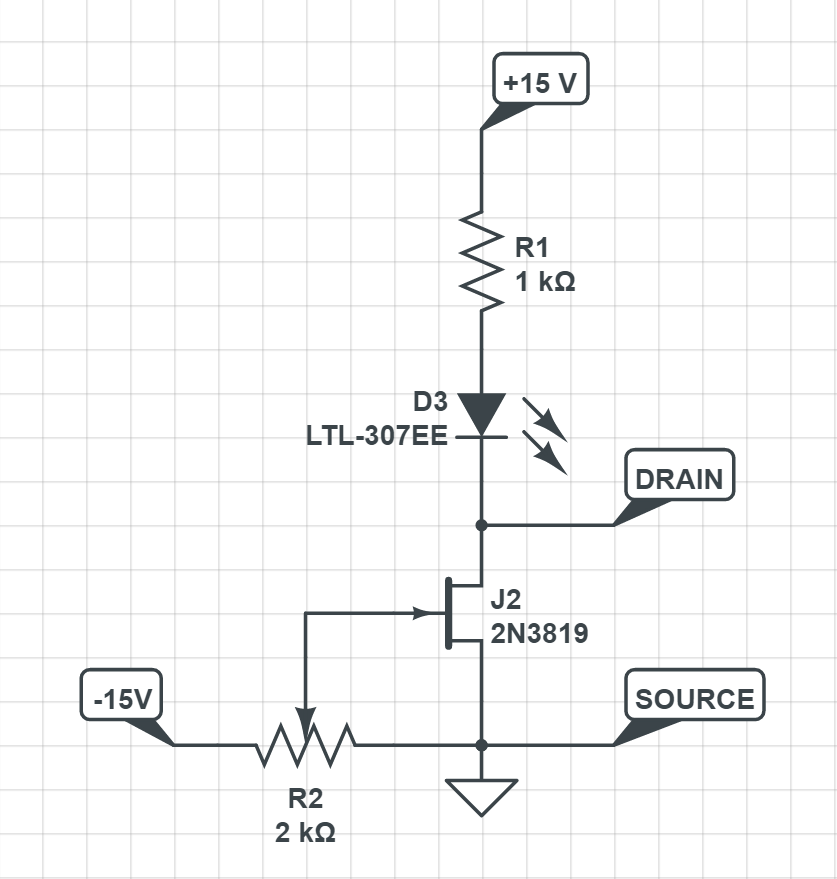
\includegraphics[scale=0.33]{firstsetup.png}
	\caption{Montaggio iniziale del circuito.}
	\label{f:setup_inizio}
\end{figure}

Si è montato il circuito come in \fig{setup_inizio}, verificando per prima cosa il passaggio del transistor da interdizione a saturazione al variare della regolazione del potenziometro (osservando l'accendersi e lo spegnersi del led). Si è dunque proceduto a registrare diversi valori di $V_{GS}$ e $I_D$ (quest'ultima mediante la misura della caduta di tensione sulla resistenza $R_1$), determinando $V_P = \SI{-4.4}{\V}$ e registrando come massima corrente di drain \SI{10.7}{\mA}. Considerando la caduta di tensione sul led ($\approx \SI{1.9}{\V}$ quando si alimenta con i \SI{+15}{\V} il led in serie ad una resistenza $\approx\SI{1}{\kohm}$; questa è una buona stima per la caduta di tensione a led acceso assumendo che la sua curva I/V sia come per tutti i diodi molto ripida oltre la tensione di soglia), si è dedotto di non riuscire con le resistenze usate a raggiungere la saturazione per $V_{GS} = 0$ (il che rende tra le altre cose impossibile la misura di $I_{DSS}$); abbiamo dunque provveduto a rimuovere il led dal circuito e sostituire la resistenza di drain con una da \SI{551 (5)}{\ohm}, ottenendo i dati riassunti in \tab{id_vgs} e mostrati in \fig{id_vgs}.

Dai dati si deduce $V_P = \SI{-4.41(3)}{\V}$, $I_{DSS} = \SI{13.83(9)}{\mA}$, rispettivamente presi come il valore di tensione di gate a cui la corrente di drain si annulla e corrente di drain osservata a tensione di gate nulla; entrambi i valori rientrano negli intervalli  indicati nel datasheet. Con la nuova resistenza si nota come valga sempre $V_{DS} > V_{GS} - V_P$\footnote{Con l'esclusione dei punti presi in interdizione, chiaramente.}, ovvero il transistor raggiunga sempre la saturazione, permettendoci di determinare $I_{DSS}$ (e di scegliere, per le misure successive, un opportuno punto di lavoro).


\begin{table}[h]
	\centering
	\begin{tabular}{ *{3}{S[table-figures-exponent = 2]} } 
		{$V_{GS}$ [\si{\V}]} & {$V_{R_1}$ [\si{\V}]} & {$I_D$ [\si{\mA}]} \\
		\midrule 
		 0.40 (10) e-3	&	7.62 (5)	&	13.83 (9)	\\ 
		-4.40 (3)	&	0.10 (10) e-3	&	0.18 (18) e-3	\\ 
		-4.42 (3)	&	0.00 (10) e-3	&	0.00 (18) e-3	\\ 
		-6.14 (4)	&	0.00 (10) e-3	&	0.00 (18) e-3	\\ 
		-3.94 (3)	&	104.1 (6) e-3	&	188.9 (11) e-3	\\ 
		-4.05 (3)	&	45.1 (3) e-3	&	81.9 (6) e-3	\\ 
		-3.56 (3)	&	0.425 (3)	&	0.771 (6)	\\ 
		-3.08 (3)	&	1.037 (6)	&	1.882 (11)	\\ 
		-2.530 (23)	&	1.918 (11)	&	3.481 (19)	\\ 
		-1.616 (9)	&	3.72 (3)	&	6.75 (5)	\\ 
		-0.992 (6)	&	5.07 (4)	&	9.20 (6)	\\ 
		-0.420 (3)	&	6.45 (4)	&	11.71 (8)	\\ 
	\end{tabular} 
	\caption{Valori registrati per tensioni e correnti variando la resistenza del potenziometro.} 
	\label{t:id_vgs} 
\end{table}

\begin{figure}[h]
	\centering
	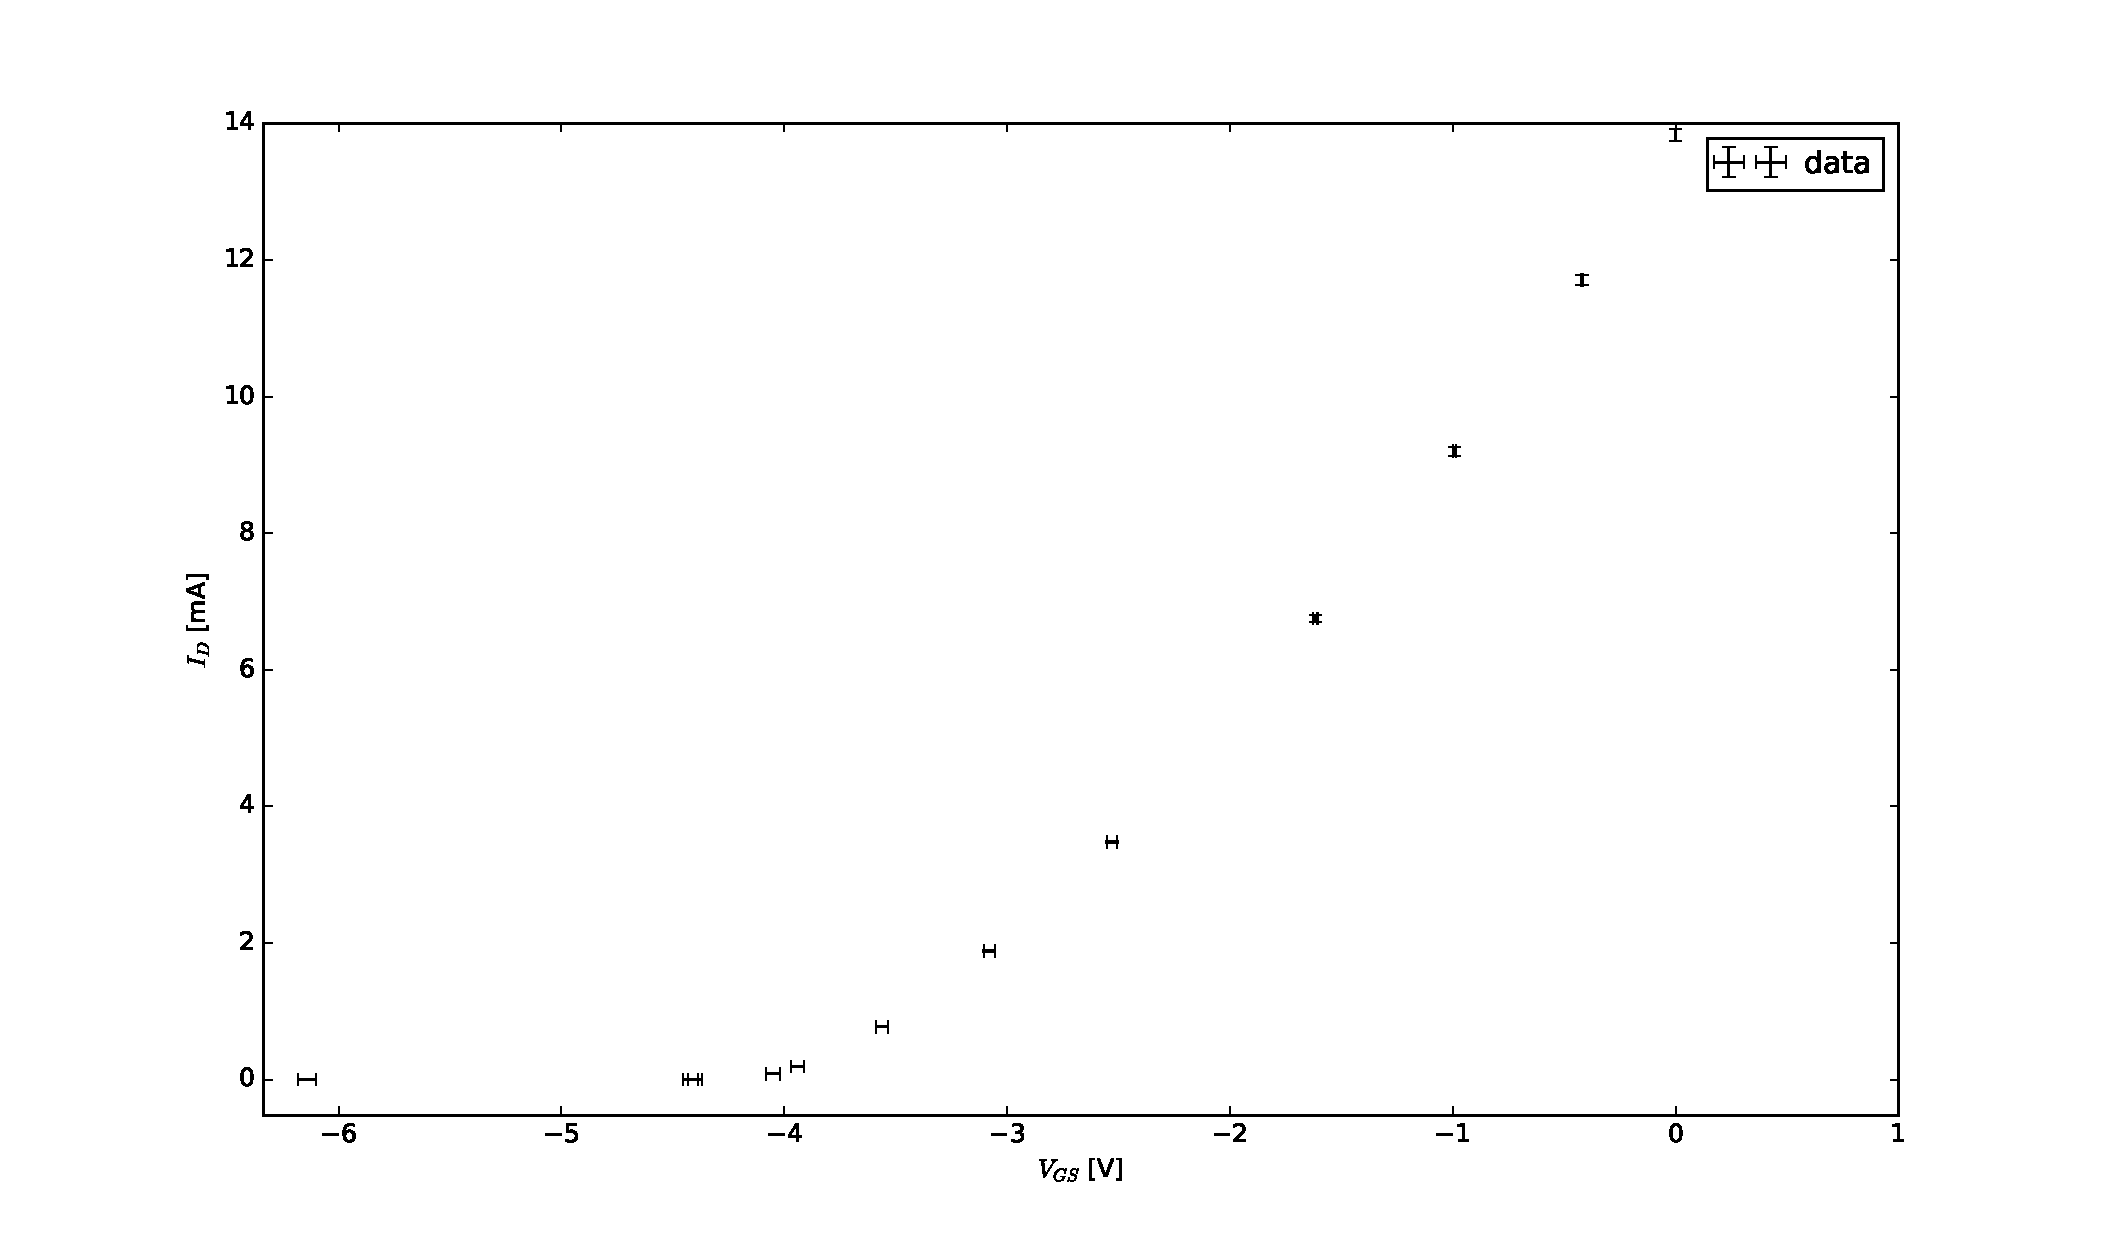
\includegraphics[scale=0.5]{1_id_vgs.pdf}
	\caption{$I_D$ contro $V_{GS}$.}
	\label{f:id_vgs}
\end{figure}